%\documentclass[10pt,flushrt,preprint]{aastex}

\documentclass[preprint]{aastex}

\usepackage{graphicx}
\usepackage[space]{grffile}
\usepackage{latexsym}
\usepackage{amsfonts,amsmath,amssymb}
\usepackage{url}
\usepackage[utf8]{inputenc}
\usepackage{fancyref}
\usepackage{hyperref}
\hypersetup{colorlinks=false,pdfborder={0 0 0},}
\usepackage{textcomp}
\usepackage{longtable}
\usepackage{multirow,booktabs}

\usepackage{natbib}

\newcommand{\truncateit}[1]{\truncate{0.8\textwidth}{#1}}
\newcommand{\scititle}[1]{\title[\truncateit{#1}]{#1}}


%% preprint2 produces a double-column, single-spaced document:

%% \documentclass[preprint2]{aastex}

%% Sometimes a paper's abstract is too long to fit on the
%% title page in preprint2 mode. When that is the case,
%% use the longabstract style option.

%% \documentclass[preprint2,longabstract]{aastex}

%% If you want to create your own macros, you can do so
%% using \newcommand. Your macros should appear before
%% the \begin{document} command.
%%
%% If you are submitting to a journal that translates manuscripts
%% into SGML, you need to follow certain guidelines when preparing
%% your macros. See the AASTeX v5.x Author Guide
%% for information.


%% You can insert a short comment on the title page using the command below.

\slugcomment{tbd journal: MNRAS}

%% If you wish, you may supply running head information, although
%% this information may be modified by the editorial offices.
%% The left head contains a list of authors,
%% usually a maximum of three (otherwise use et al.).  The right
%% head is a modified title of up to roughly 44 characters.
%% Running heads will not print in the manuscript style.

\shorttitle{The MWA Epoch of Reionization Project: Summary of Results}
\shortauthors{D. Jacobs}

%% This is the end of the preamble.  Indicate the beginning of the
%% paper itself with \begin{document}.


%% Use \author, \affil, and the \and command to format
%% author and affiliation information.
%% Note that \email has replaced the old \authoremail command
%% from AASTeX v4.0. You can use \email to mark an email address
%% anywhere in the paper, not just in the front matter.
%% As in the title, use \\ to force line breaks.
\def\eppsilon{{\it $\epsilon$ppsilon }}
\def\empirical cov{\emph{EMPCOV }}
\def\chipscite{Trott et al 2015}
\def\eppsiloncite{Hazelton et al 2015}
\def\dilloncite{Dillon et al 2015}




\def\ASU{\altaffilmark{1}}
\def\ASUtxt{\altaffiltext{1}{Arizona State University, School of Earth and Space Exploration, Tempe, AZ 85287, USA}}

\def\myemail{\altaffilmark{*}}
\def\myemailtxt{\altaffiltext{*}{e-mail: daniel.c.jacobs@asu.edu}}

\def\UW{\altaffilmark{2}}
\def\UWtxt{\altaffiltext{2}{University of Washington, Department of Physics, Seattle, WA 98195, USA}}

\def\SKASA{\altaffilmark{3}}
\def\SKASAtxt{\altaffiltext{3}{Square Kilometre Array South Africa (SKA SA), Park Road, Pinelands 7405, South Africa}}

\def\RU{\altaffilmark{4}}
\def\RUtxt{\altaffiltext{4}{Department of Physics and Electronics, Rhodes University, Grahamstown 6140, South Africa}}

\def\CfA{\altaffilmark{5}}
\def\CfAtxt{\altaffiltext{5}{Harvard-Smithsonian Center for Astrophysics, Cambridge, MA 02138, USA}}

\def\ANU{\altaffilmark{6}}
\def\ANUtxt{\altaffiltext{6}{Australian National University, Research School of Astronomy and Astrophysics, Canberra, ACT 2611, Australia}}

\def\CAASTRO{\altaffilmark{7}}
\def\CAASTROtxt{\altaffiltext{7}{ARC Centre of Excellence for All-sky Astrophysics (CAASTRO)}}

\def\Haystack{\altaffilmark{8}}
\def\Haystacktxt{\altaffiltext{8}{MIT Haystack Observatory, Westford, MA 01886, USA}}

\def\MIT{\altaffilmark{9}}
\def\MITtxt{\altaffiltext{9}{MIT Kavli Institute for Astrophysics and Space Research, Cambridge, MA 02139, USA}}

\def\Curtin{\altaffilmark{10}}
\def\Curtintxt{\altaffiltext{10}{International Centre for Radio Astronomy Research, Curtin University, Perth, WA 6845, Australia}}

\def\Victoria{\altaffilmark{11}}
\def\Victoriatxt{\altaffiltext{11}{Victoria University of Wellington, School of Chemical \& Physical Sciences, Wellington 6140, New Zealand}}

\def\UWisc{\altaffilmark{12}}
\def\UWisctxt{\altaffiltext{12}{University of Wisconsin--Milwaukee, Department of Physics, Milwaukee, WI 53201, USA}}

\def\UMichigan{\altaffilmark{13}}
\def\UMichigantxt{\altaffiltext{13}{University of Michigan, Department of Atmospheric, Oceanic and Space Sciences, Ann Arbor, MI 48109, USA}}

\def\UMelbourne{\altaffilmark{14}}
\def\UMelbournetxt{\altaffiltext{14}{The University of Melbourne, School of Physics, Parkville, VIC 3010, Australia}}

\def\USydney{\altaffilmark{15}}
\def\USydneytxt{\altaffiltext{15}{The University of Sydney, Sydney Institute for Astronomy, School of Physics, NSW 2006, Australia}}

\def\CASS{\altaffilmark{16}}
\def\CASStxt{\altaffiltext{16}{CSIRO Astronomy and Space Science (CASS), PO Box 76, Epping, NSW 1710, Australia}}

\def\Tata{\altaffilmark{17}}
\def\Tatatxt{\altaffiltext{17}{National Centre for Radio Astrophysics, Tata Institute for Fundamental Research, Pune 411007, India}}

\def\RRI{\altaffilmark{18}}
\def\RRItxt{\altaffiltext{18}{Raman Research Institute, Bangalore 560080, India}}

\def\NRAO{\altaffilmark{19}}
\def\NRAOtxt{\altaffiltext{19}{National Radio Astronomy Observatory, Charlottesville and Greenbank, USA}}

\def\UWA{\altaffilmark{20}}
\def\UWAtxt{\altaffiltext{20}{International Centre for Radio Astronomy Research, University of Western Australia, Crawley, WA 6009, Australia}}

%% \definenote[thanks][conversion=set 2]

\begin{document}

%% LaTeX will automatically break titles if they run longer than
%% one line. However, you may use \\ to force a line break if
%% you desire.

\title{The Murchison Widefield Array Epoch of Reionization Pipelines}


%% Use \author, \affil, and the \and command to format
%% author and affiliation information.
%% Note that \email has replaced the old \authoremail command
%% from AASTeX v4.0. You can use \email to mark an email address
%% anywhere in the paper, not just in the front matter.
%% As in the title, use \\ to force line breaks.

%% Author list
\author{
%% Lead Authors
Daniel~C.~Jacobs\ASU\myemail,
N.~Barry\UW,
A.~P.~Beardsley\UW,
G.~Bernardi\SKASA$^,$\RU$^,$\CfA,
Judd~D.~Bowman\ASU,
F.~Briggs\ANU$^,$\CAASTRO,
R.~J.~Cappallo\Haystack, 
P.~Carroll\UW,
B.~E.~Corey\Haystack, 
% A.~A.~Deshpande\RRI, 
A.~de~Oliveira-Costa\MIT,
Joshua~S.~Dillon\MIT,
D.~Emrich\Curtin,
 B.~M.~Gaensler\USydney$^,$\CAASTRO, 
A.~Ewall-Wice\MIT,
L.~Feng\MIT,
R.~Goeke\MIT,
L.~J.~Greenhill\CfA,
B.~J.~Hazelton\UW, 
J.~N.~Hewitt\MIT,
N.~Hurley-Walker\Curtin,
M.~Johnston-Hollitt\Victoria,
D.~L.~Kaplan\UWisc, 
J.~C.~Kasper\UMichigan$^,$\CfA, 
Han-Seek Kim\UMelbourne$^,$\CAASTRO,
P.~Kittiwisit\ASU,
E.~Kratzenberg\Haystack, 
E.~Lenc\USydney$^,$\CAASTRO,
J.~Line\UMelbourne$^,$\CAASTRO,
A.~Loeb\CfA,
C.~J.~Lonsdale\Haystack, 
M.~J.~Lynch\Curtin, 
B.~McKinley\UMelbourne$^,$\CAASTRO,
S.~R.~McWhirter\Haystack,
D.~A.~Mitchell\CASS$^,$\CAASTRO, 
M.~F.~Morales\UW, 
E.~Morgan\MIT, 
A.~R.~Neben\MIT,
Nithyanandan~Thyagarajan\ASU,
D.~Oberoi\Tata, 
A.~R.~Offringa\ANU$^,$\CAASTRO, 
S.~M.~Ord\Curtin$^,$\CAASTRO,
Sourabh Paul\RRI,
B.~Pindor\UMelbourne$^,$\CAASTRO,
J.~C.~Pober\UW,
T.~Prabu\RRI, 
P.~Procopio\UMelbourne$^,$\CAASTRO,
J.~Riding\UMelbourne$^,$\CAASTRO,
A.~E.~E.~Rogers\Haystack, 
A.~Roshi\NRAO, 
N.~Udaya~Shankar\RRI, 
Shiv~K.~Sethi\RRI,
K.~S.~Srivani\RRI, 
R.~Subrahmanyan\RRI$^,$\CAASTRO, 
I.~S.~Sullivan\UW,
M.~Tegmark\MIT,
S.~J.~Tingay\Curtin$^,$\CAASTRO, 
C.~M.~Trott\Curtin$^,$\CAASTRO,
M.~Waterson\Curtin$^,$\ANU,
R.~B.~Wayth\Curtin$^,$\CAASTRO, 
R.~L.~Webster\UMelbourne$^,$\CAASTRO, 
A.~R.~Whitney\Haystack, 
A.~Williams\Curtin, 
C.~L.~Williams\MIT,
C.~Wu\UWA,
J.~S.~B.~Wyithe\UMelbourne$^,$\CAASTRO
}

%Institutional footnotes (typeset, then rearrange here to be in order)
\ASUtxt
\myemailtxt
\UWtxt
\SKASAtxt
\RUtxt
\CfAtxt
\ANUtxt
\CAASTROtxt
\Haystacktxt
\MITtxt
\Curtintxt
\Victoriatxt
\UWisctxt
\UMichigantxt
\UMelbournetxt
\USydneytxt
\CASStxt
\Tatatxt
\RRItxt
\NRAOtxt
\UWAtxt



%\author{
%Danny Jacobs\altaffilmark{1},
%Ian Sullivan \altaffilmark{2}
%Bryna Hazelton \altaffilmark{2},
%Bart Pindor \altaffilmark{3},
%Cath Trott \altaffilmark{4},
%Josh Dillon \altaffilmark{5},
%Abraham Neben \altaffilmark{5},
%Adam Beardsley \altaffilmark{2},
%EoR list,
%Builders list
%}
%\altaffiltext{1}{School of Earth and Space Exploration, Arizona State U., Tempe, AZ}
%\altaffiltext{2}{Physics Dept. University of Washington, Seattle, WA}
%\altaffiltext{3}{Melbourne University, Melbourne, Aus}
%\altaffiltext{4}{Curtin University, Perth, Aus}
%\altaffiltext{5}{Massachusetts Institute of Technology, Boston, MA}
\begin{abstract}
We present an overview of the Murchison Widefield Array 21\,cm Epoch of Reionization analysis methods in which we compare the output of multiple pipelines as applied to a representative selection of data. The focus of this first round of analysis is on building the methodological foundation for detecting the weak statistical signature of cosmological HI at redshifts 6 to 10 in multi-year MWA observations. This paper provides a top level view over the methods and results of multiple, independent, data calibration and reduction pipelines.  To assess the accuracy of our methods we split the data analysis steps into the two steps widely considered to present the most challenges, bright foreground removal and power spectrum estimation in the presence of residual foregrounds.  Comparing images we see agreement on a significant amount of large scale, galactic, structure, though small differences related to calibration and weighting remain. Features common to all power spectrum results show the continued significance of wide-field effects, while differences in both imaging and power spectrum convey the importance of calibration algorithms and point towards future work. Using the calibrated and integrated image cubes we apply an inverse covariance technique to make a noise limited estimate of the power spectrum.   %Using the calibration refined through repeated  estimates of the power spectrum, a method itself calibrated against both models and independent reductions, in combination with down-weighting of residual covariance, we arrive at a noise limited power spectrum.


%The Murchison Widefield Array (MWA) in Western Australia is currently
%performing thousand hour integrations in the 2~m radio band with the
%goal of detecting redshifted 21~cm emission from the Epoch of
%Reionization (EoR) when the first stars are expected to reionize the
%universe on cosmological scales. Our goal is to observe the power
%spectrum of inter-galactic hydrogen as reionization proceeds and
%constrain the timing and speed of this key step in the universe's
%development. Because deep 21~cm power spectrum observations are very new
%and require unprecedented levels of precision and foreground removal, we
%have developed multiple analysis pipelines with redundant cross-checking
%at each major processing stage to increase our confidence in the
%reliability of the analysis. In this paper we describe the two parallel
%analysis pipelines that will be used to analyze the MWA EoR data and
%present initial power spectra and quality checks from the first nights
%of EoR observing with the full MWA instrument.

\end{abstract}




%% Keywords should appear after the \end{abstract} command. The uncommented
%% example has been keyed in ApJ style. See the instructions to authors
%% for the journal to which you are submitting your paper to determine
%% what keyword punctuation is appropriate.

%\keywords{globular clusters: general --- globular clusters: individual(NGC 6397, NGC 6624, NGC 7078, Terzan 8}

\bibliographystyle{apj_w_etal}


\section{Introduction} 
  Study of intergalactic Hydrogen  in the early universe via the 21\,cm line is forecast to provide a wealth of astrophysical and cosmological information.  The 21\,cm line is both optically thin and spectrally narrow, making possible full tomographic reconstruction. Cosmological Hydrogen is neutral over cosmic time from recombination until reionized by the first batch of UV emitters (stars and accretion disks).  Reviews of 21 cm cosmology, astrophysics and observing can be found in \cite{Morales:2010p8093,Furlanetto:2006p2267,Pritchard:2012p9555,zaroubi2013epoch}.
  
Direct detection of HI during the Epoch of Reionization (cosmological redshifts $5<z<13$) is currently the goal of several new radio arrays. The LOw Frequency ARray \citep[LOFAR;]{Yatawatta:2013p9699}, the Donald C. Backer Precision Array for Probing the Epoch of Reionization (PAPER; \citet{Parsons:2014p10499}) and the Murchison Widefield Array (MWA; \cite{Tingay:2013p9022,Bowman:2013p9950}) are all currently conducting long observing campaigns.

The analysis of the resulting data presents several challenges. The signal is faint; initial detection is being sought in the power spectrum with thousands of hours (multiple seasons) of integration required. This faint spectral line signal sits atop a continuum foreground four orders of magnitude brighter. At the same time, the instruments are fully correlated phased arrays with wide fields of view that strain the conventional mathematical assumptions of radio astronomy practice. The methods used to arrive at a well calibrated, foreground-free, estimation of the power spectrum are all under development in the sense of the algorithms as well as the implementation.  


The path from observation to power spectrum can be roughly divided into two parts: removal of foregrounds and estimation of power spectrum.  Recently two sorts of foreground removal have been suggested. Blind filtering, such as the delay/fringe-rate filtering approach \citep{Parsons:2012p8896,Liu:2014p10462,Liu:2014p10463},  that has been applied to data from the PAPER telescope \citep{Parsons:2014p10499}, applies a small amount of knowledge about the instrument to filter modes likely to be contaminated.  This method is comparatively robust in the face of uncertainty about the instrument and the sky, at the cost of losing some sensitivity. Meanwhile,  full forward modeling and subtraction of sky model such as that implemented for LOFAR (see e.g. \cite{Jelic:2008p2130,Yatawatta:2013p9699}), requires a much higher fidelity model of the instrument and the sky \citep{Datta:2010p8781,Vedantham:2012p10297}.  

The MWA analysis approach focuses on direct subtraction of known foregrounds.  If successful, it has the benefit of opening the most sensitive power spectrum modes within the ``wedge'' and substantially improving the ability of early measurements to distinguish between reionization models \citep{Beardsley:2013p9952,Pober:2014p10390}. Recent work towards the goal of foreground subtraction includes better algorithmic handling of wide field imaging effects \citep{Tasse:2012p9459,Bhatnagar..2013ApJ,Sullivan:2012p9457,Ord:2010p8442}, and continually improving catalogs of sky emission \citep{deOliveiraCosta:2008p2242,Jacobs:2011p8438,Hurley-walker:2014p45,2014AAS...22342101M}. Ongoing operation of the next generation low frequency arrays --LOFAR, PAPER and MWA are all in their second or third year of operation-- continues to push the refinement instrumental models (e.g. the work of \cite{Neben:2015pxxx} in mapping the primary beam with satellites) and improve the accuracy of model subtraction.  At the same time, more complete surveys of 21\,cm reionization foregrounds are currently under way. These include the MWA GLEAM\footnote{GLEAM: Galactic and Extragalactic All-sky MWA} survey  and the LOFAR MSSS\footnote{MSSS: Multi-frequency Snapshot Sky Survey}.   %todo insert MWACS cite when available



Given the challenges of using newly developed methods to reduce data from a novel instrument to make a low sensitivity detection, it is reasonable to consider the question of how one knows one is getting the ``right'' answer.  One option is to generate, as accurately as possible, a detailed simulation of the interferometer output. Full instrument simulation is computationally demanding and difficult to divorce from the analysis methods being tested, which at their core are instrument simulation engines. Development of a completely independent instrumental simulation and is the subject of ongoing work \citep[see e.g..][]{2015arXiv150207596T}, but is not available at scale at this time.  The second option is more pragmatic; compare the results of multiple independent pipelines.  

Within the MWA collaboration efforts have centered around two, completely independent, paths from raw data to a power spectrum.  In this paper we outline each method, leaving the detailed descriptions to other papers.   The first pipeline uses Fast Holographic Deconvolution (FHD\footnote{\url{github.com/miguelfmorales/FHD}}) for calibration and foreground subtraction, followed by either \eppsilon\footnote{\eppsilon:Error Propagated Power Spectrum with InterLeaved Observed Noise;} or \empirical cov to estimate the power spectrum.  The second pipeline uses an offline version of the MWA Real Time System (RTS) followed by CHIPS\footnote{Cosmological HI Power Spectrum} to estimate the power spectrum.  FHD is described in detail by \cite{Sullivan:2012p9457} and the RTS by \cite{Ord:2010p8442}. \eppsilon, CHIPS and \empirical cov, as applied to the data published here, are described in \eppsiloncite, \chipscite, and \dilloncite, respectively.

One benefit from having multiple pipelines is the freedom to focus on different optimization axes.  The design of the \eppsilon power spectrum estimator emphasizes speed and relative sempirical y, choices  motivated by the need to understand the effect of processing decisions such as observation protocol, flagging, and calibration on the {\bf power spectrum}. Using \eppsilon we have discovered and corrected multiple systematic effects visible only in the power spectrum. With the ability to quickly form power spectra on different sets of data \eppsilon has been our primary method for selecting sets of high quality data. Whereas both \eppsilon and CHIPS operate on time-ordered data, \empirical cov takes as input single cubes of integrated data (one each for even and odd time samples) which have been selected on the basis statistics like interference and calibration quality and curation with \eppsilon. The \empirical cov method uses an empirical estimate of the instrumental covariance to mitigate any remaining residual in the Fourier modes due to instrument mismodeling in the previous steps. 

 The MWA EoR program has collected more than 1000 hours of data but here we will limit ourselves to a single night (3 hours) an amount which is sufficient to gain insight into the net performance of our calibration algorithms and foreground subtraction models without adding the complexity of a large dataset.  Upcoming analyses will focus on going deeper, using analysis techniques built upon the foundation methods described here and in the companion papers.

In \ref{sec:observing} we summarize the observing strategy used to collect our data, \ref{sec:pipelines} explains our multiple pipelines and comparison strategy. In section \ref{sec:results} we show comparisons of images, 2D diagnostic power spectra and 1D power spectrum limits, and conclude in section \ref{sec:conclusion} with an overview of lessons learned from the comparison process and directions of future work .


%\section{Pipeline overview}
%\label{sec:overview}
%Within the MWA reionization pipelines foreground removal is handled either by Full Holographic Deconvolution \citep[FHD]{Sullivan:2012p9457}\footnote{\url{github.com/miguelfmorales/FHD}} or the Real Time System \citep[RTS]{Ord:2010p8442}.  Here we use FHD to refer to a specific implementation of the algorithm constructed primarily for the reduction of MWA data, though it has been successfully applied to data from other telescopes.  The RTS is a hardware/software solution, originally designed to support operation of online imaging of the 512 element MWA, that has been repurposed and expanded into a general imaging package suitable for offline data reduction.
%
%
% Estimation of the power spectrum that takes into account instrumental and sky uncertainty can also ameliorate some of the conflict between foreground and background.  Power spectrum estimation methods include \eppsilon\footnote{\eppsilon:Error Propagated Power Spectrum with InterLeaved Observed Noise;} \eppsiloncite, CHIPS\footnote{Cosmological HI Power Spectrum} \chipscite and \empirical cov \dilloncite.
% 
% \eppsilon  operates on residual images and is optimized for speed and error propagation. In simulation, the \eppsilon $+$ FHD combination has uncovered new mode-mixing features in the foreground power spectrum \citep{Morales:2012p8790}.  Trott et al have implemented CHIPS which uses an optimal estimator approach (e.g. \cite{Liu:2011p8763})  that operates directly on the time-ordered visibilities which have had an initial round of foreground subtraction.  In a second implementation of the optimal estimator approach \dilloncite takes image cubes produced by FHD and curated by \eppsilon, and uses an empirical calculation of foreground covariance to further down-weight foregrounds and place noise-limited estimates on the power spectrum.




\section{Observing}
\label{sec:observing}
The MWA is an an interferometric array of phased array tiles operating in the 80-300\,MHz radio band. Each tile consists of a 4x4 grid of bow-tie shaped dipoles that are used to form a beam on the sky, steered by an analog delay-line beamformer.  The signal is digitized over the entire bandwidth but only 30\,MHz are available at any one time.  This 30\,MHz of bandwidth is broken into 1.28\,MHz ``coarse'' bands by a polyphase filter-bank in the field and sent to the correlator where it is further channelized to 40kHz, cross-correlated and then averaged at 0.5 second intervals. The spectral shape of the coarse polyphase filter is known somewhat imperfectly and is thought to include a small amount of aliasing from adjacent coarse channels, though the exact amount is currently under investigation. This spectral response is corrected to first order during the first post-correlator step, and to second order by the calibration step.  More details on the design and operation of the MWA can be found in \cite{Lonsdale:2009p7913} and \cite{Tingay:2013p9022}.

The MWA EoR observing scheme focuses on two 30\,MHz tunings, 140-170\,MHz and 167-196\,MHz (so-called 'low' and 'high') and two minimal foreground regions both -27\arcdeg declination (near zenith at the MWA's latitude) at RA 0h and 4h (referred to as EoR0 and EoR1). Here we focus on the 'high' tuning pointing at EoR0, where the high band is chosen for its low sky temperature and EoR0 is chosen for its ease of calibration (lacking bright, resolved sources). During observing, the beam former was set such that the target region repeatedly drifted over the beam.  Each drift was about 30 minutes long.  This was done for a total of 6 pointings in a night, or about 3 hours. The data included here include the two pointings leading up to the target crossing zenith, the zenith pointing, and then three more pointings after the transit crossing.  Data were recorded in 112 second units for a total of 98 snapshots. These snapshots are the basic unit of time on which many operations become independent -eg RFI flagging, FHD calibration and imaging.\footnote{Note that this is not true in the RTS case which uses a time interval scaled by the baseline length.}   Each snapshot is flagged for interference using the AOFlagger\footnote{\url{sourceforge.net/projects/aoflagger}} algorithm and then averaged to 2 seconds and 80kHz.  As described in \cite{2015PASA...32....8O}, the interference environment at the Murchison Observatory is benign and generally requires flagging of about 1\% of the data.   Though the full set of linear stokes parameters are correlated, and Stokes I images and power spectra are the final product of interest, at this stage of the analysis the instrumental polarizations have been found to be more instructive; only the linear X (east-west) polarization is examined here.  

\begin{deluxetable}{lcr}
\tablecolumns{3}
\tablecaption{MWA EoR Observing Parameters }
\tablehead{
\colhead{parameter}  & 
\colhead{value} &
\colhead{notes}
}
\startdata
field of view & 26\arcdeg & FWHM, scales as $\lambda$ \tabularnewline
tuning & 166-196\,MHz & redshift range $7.56<z<6.25$ \tabularnewline
target area & (RA,Dec) 0h00m, -27\arcdeg00m & \tabularnewline
pointing seperation & 6.8\arcdeg & \tabularnewline
time and frequency resolution & 0.5\,s, 40 kHz &  \tabularnewline
post-flagging resolution & 2s, 80\,kHz & \tabularnewline
time & 3 hours on August 23, 2013 & a total of 6 pointings, lasting 30m each \tabularnewline
\enddata
\label{tab:observing}
\end{deluxetable}


%The MWA has observed 350 hours during the Fall 2013 EoR season.  The two main observing variables are choice of 30MHz band and pointing. Total time is limited. Observations are thermal noise limited. After about 1000 hours on a particular sky location and tuning they become cosmic variance limited.   






\section{Power Spectrum Pipelines}
\label{sec:pipelines}



  There are many possible paths to a detection of 21\,cm reionization but all must in some way remove foregrounds and compute an estimate of the power spectrum\footnote{or some similar statistical measure} . In subtracting a foreground model one must account for:  ionospheric distortion, very wide field, primary beam uncertainty, polarization leakage, and calibration accuracy. The MWA pipeline has two independent calibration and imaging modules which subtract the foregrounds and two power spectrum estimators. All are developed independently, sharing very little code, yet are interconnectable via common data formats to give four possible pipeline paths.These two paths and their interactions are sketched out in Figure \ref{fig:pipes}.


The imaging and foreground subtraction portion of the pipeline can be handled by either of two custom packages.  The MWA Real Time System (RTS; \cite{Ord:2010p8442}) was initially designed to make images in real time from the MWA 512.  On the de-scoped 128 element array, it has been implemented as an offline system, where it has been adjusted to compensate for the lower filling factor.  Fast Holographic Deconvolution (FHD; \cite{Sullivan:2012p9457}) is a custom interferometric imaging package developed for wide-field instruments with a focus on accounting for the very wide field of view antenna responses found on phased arrays of dipoles.  Both systems were developed in parallel with the construction and commissioning of the MWA to provide a detailed introspection on every aspect of this experimental telescope. Each can calibrate a data set against a model, subtract a model, deconvolve images and use precision models of the instrument informed by the commissioning process including effects such as tile to tile primary beam variation and 0.1dB cable reflections.  Foreground inputs include catalogs, images of extended emission and wavelet models of bright, mostly compact, sources.  In addition, each has its own unique feature set developed as part of the experimental process.

\begin{figure*}[htbp]
\begin{center}
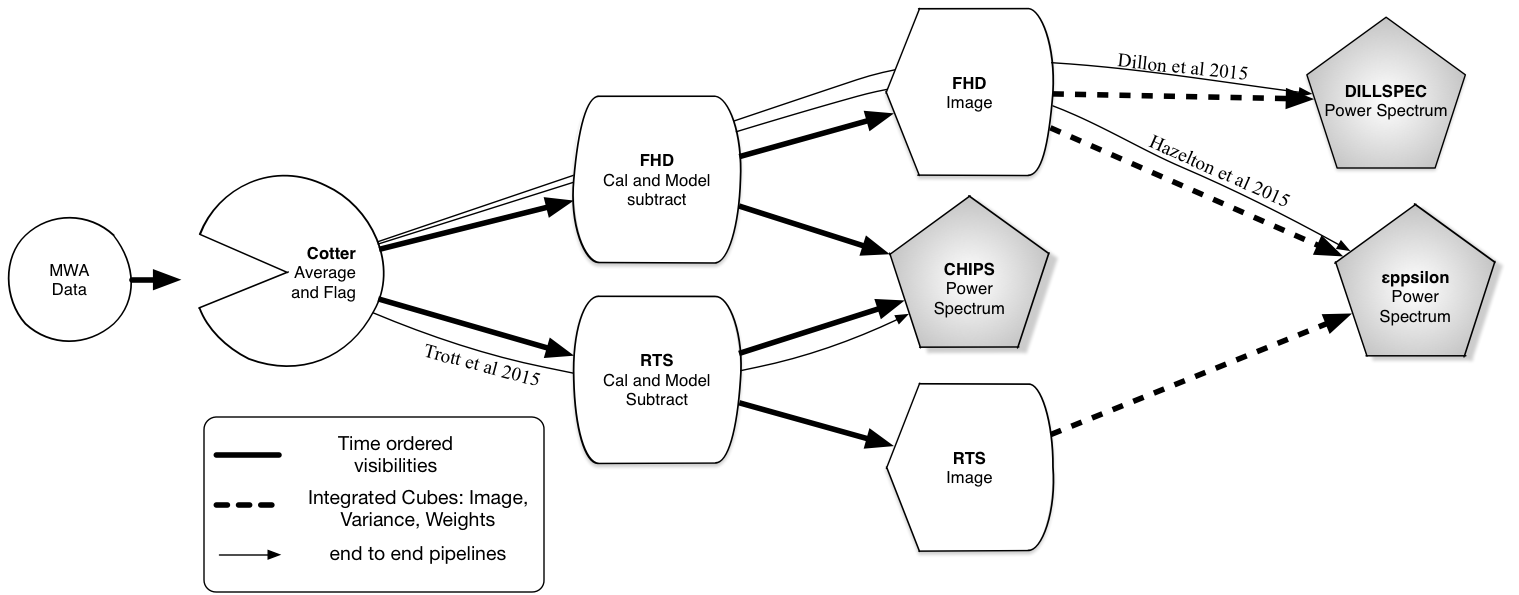
\includegraphics[width=\textwidth]{figures/MWA_Pipes.png}
\caption{Parallel pipelines with cross-connections after foreground subtraction and imaging are compared against each other as a guard against error.  Cotter uses AOFlagger to flag RFI and averages by a factor of 8. The averaged snapshots are passed to either FHD or RTS for calibration and imaging, \eppsilon takes the resulting snapshots, averages them in LST and estimates the power spectrum. CHIPS taps into the RTS and FHD to get calibrated and foreground subtracted time-ordered (not yet gridded) visibilities which it then uses to make its own estimate of the power spectrum. }
\label{fig:pipes}
\end{center}
\end{figure*}

\subsection{Calibration and Imager \#1: RTS}
\label{sec:RTS}
The MWA Real Time System (RTS) is a radio interferometry software package specifically written to calibrate and image MWA data \citep[][Mitchell et al. in prep]{Ord:2010p7534}. The RTS incorporates algorithms intended to address a number of known challenges inherent to processing MWA data, including; wide-field imaging effects, direction-dependant (DD) antenna gains and polarization response, and ionospheric refraction of low-frequency radio waves. Each MWA observation (112s) is processed through a separate instance of the RTS. The RTS is also parallelized over frequency so that each coarse channel (1.28\,MHz broken into 40 kHz channels) is processed largely independently of the other coarse channels, with only information about the measured ionospheric offsets communicated between processing nodes.  Calibration and model subtraction were based on the TBD catalog. 

The RTS calibration strategy is based upon the 'Peeling' technique proposed by \cite{Noordam:2004p2379}. The brightest (apparent) radio sources in the field of view are sequentially and iteratively processed through a Calibrator Measurement Loop (CML). During each pass through the CML; i) the expected (model) visibilities of known catalogue sources are subtracted from the observed visibilities. For the data processed in this work, $\sim$100 sources are subtracted for each observation. ii) The model visibilites for the targeted source are added back in and phased to the catalog source location. Any ionospheric offset of the source can now be measured by fitting a phase ramp to the phased visibilities. iii) The strongest sources are now used to update the direction-dependant antenna gain terms, while weaker sources are only corrected for ionospheric offsets. For this work, TBD sources are used as full DD calibrators and 100 sources are set as ionospheric calibrators. The CML is repeated until the gain and ionospheric fits converge to stable values. The $\sim$100 strongest sources are then subtracted from the calibrated visibilities and the residuals are passed to the visibility-based power spectrum described in Section \ref{sec:CHIPS} and shown in Figure \ref{fig:pspec_compare}.  A single bandpass for each tile is found by fitting a 2nd order polynomial to each coarse channel. Calibration and model subtraction parameters are summarized in Table \ref{tab:cal_sub_parms}.  Model subtracted visibilities are passed to the RTS imager and to the CHIPS power spectrum estimator. %how much flux is subtracted in total?

The RTS uses a snapshot imaging approach to correct for wide-field and direction-dependant polarization effects. Following calibration, the residual visibilities are first gridded to form instrumental polarization images which are co-planar with the array. These images are then regridded into the HEALPIX frame with wide-field corrections and conversion to Stokes applied through the regridding weights. It is also possible to use the fitted ionospheric calibrator offsets to apply a correction for ionospheric effects across the field during the regridding step, but in this work this correction has not been applied. See \citet{Clark_Allen_Arcus_et_al__2010} for a more complete description of the RTS imaging algorithms.  The resulting image spectral cubes, output on a 112s cadence paired with a spectral image cube of the point-spread function (Fourier dual to the weights in the $uvf$ plane), and the variance (dual to the $uvf$ weights squared).  The mean of the image cube is shown in Figure \ref{fig:image_compare}, power spectra of with RTS foreground subtraction are shown in the bottom row of Figure \ref{fig:pspec_compare}.
\begin{deluxetable}{lcr}
\tablecolumns{3}
\tablecaption{MWA EoR Calibration and Model subtraction Parameters }
\tablehead{
\colhead{parameter}  & 
\colhead{value} &
\colhead{free parameters}
}
\startdata
&RTS&\tabularnewline
\hline
passband & 2nd order poly per coarse channel & 48 per tile  \tabularnewline
gain & amplitude and phase & 2 per tile \tabularnewline
Direction Dependent & 2x2 Jones matrix & 4 per DD source  \tabularnewline
Catalog &TBD& \tabularnewline
sources subtracted & TBD& TBD flux cut\tabularnewline 
\tabularnewline
& FHD & \tabularnewline
\hline
passband & fine channel gain spectrum & 768 channels for entire array \tabularnewline
passband & 2nd order poly over full band (1st order for phase) & 3 per tile\tabularnewline
gain & amplitude and phase & 2 per tile\tabularnewline
Catalog &MWA Commissioning Survey& \tabularnewline
sources subtracted & 1000&TBD flux cut\tabularnewline 
\enddata
\label{tab:cal_sub_parms}
\end{deluxetable}

\subsection{Imager \#2: FHD}
Fast Holographic Deconvolution (FHD, \cite{Sullivan:2012p9457}) is a calibration and imaging algorithm designed for very wide field of view interferometers with direction- and antenna-dependent beam patterns. FHD has particularly been designed with a focus on producing an accurate measurement of the power spectrum and takes care to export the instrument model to the power spectrum estimation stage for the purposes of error propagation. Like the RTS, FHD uses the  beam pattern for gridding visibilities to the u-v plane, and its Hermitian conjugate for de-gridding simulations to form model visibilities. The  beam model is composed of the measured antenna response to the electric field for each antenna element and at every fine frequency channel, convolved with the response of the second antenna that forms the visibility. Three data outputs are necessary from gridding in order to calculate the image based power spectrum with accurate error bars: the measured visibilities, gridded with the  beam model\footnote{Note that the resulting image will be tapered by the average primary beam squared}; the weights, obtained by gridding the  beam model; and the variance, obtained by gridding the squared beam model.

The FHD calibration pipeline both measures and removes foregrounds. The calibration model is formed from sources found by deconvolving hundreds of snapshots on the EoR0 field and retaining those common to most of them.  This catalog  in the MWACS catalog having a primary beam response of 5\% or more. Solutions are then computed using the Alternating Direction Implicit technique described in \citet{sal14}.  This generates a gain and phase for every channel on every tile, for each 112s snapshot.  These solutions are then averaged over all tiles to form a single passband, which corrects for the majority of the spectral dependent effects such as the response of the coarse channel passband.  This single passband solution is then divided out of each per tile solution and each residual fit for a 2nd order amplitude polynomial and a first order phase polynomial. This process happens iteratively, with convergence measured by comparing the relative difference between residual visibilities. 10 iterations to converge to a stable residual was the norm. The residual time-ordered visibilites are then passed to CHIPS and to FHD imaging for formation of spectral cubes.  FHD splits the samples into even and odd time intervals at a 4s cadence to produce two sets of image and weight cubes which are sent to \eppsilon for power spectrum estimation.  Power spectra with FHD foreground subtraction are shown in the top row of Figure \ref{fig:pspec_compare}.


\begin{figure*}[htb]
\begin{center}
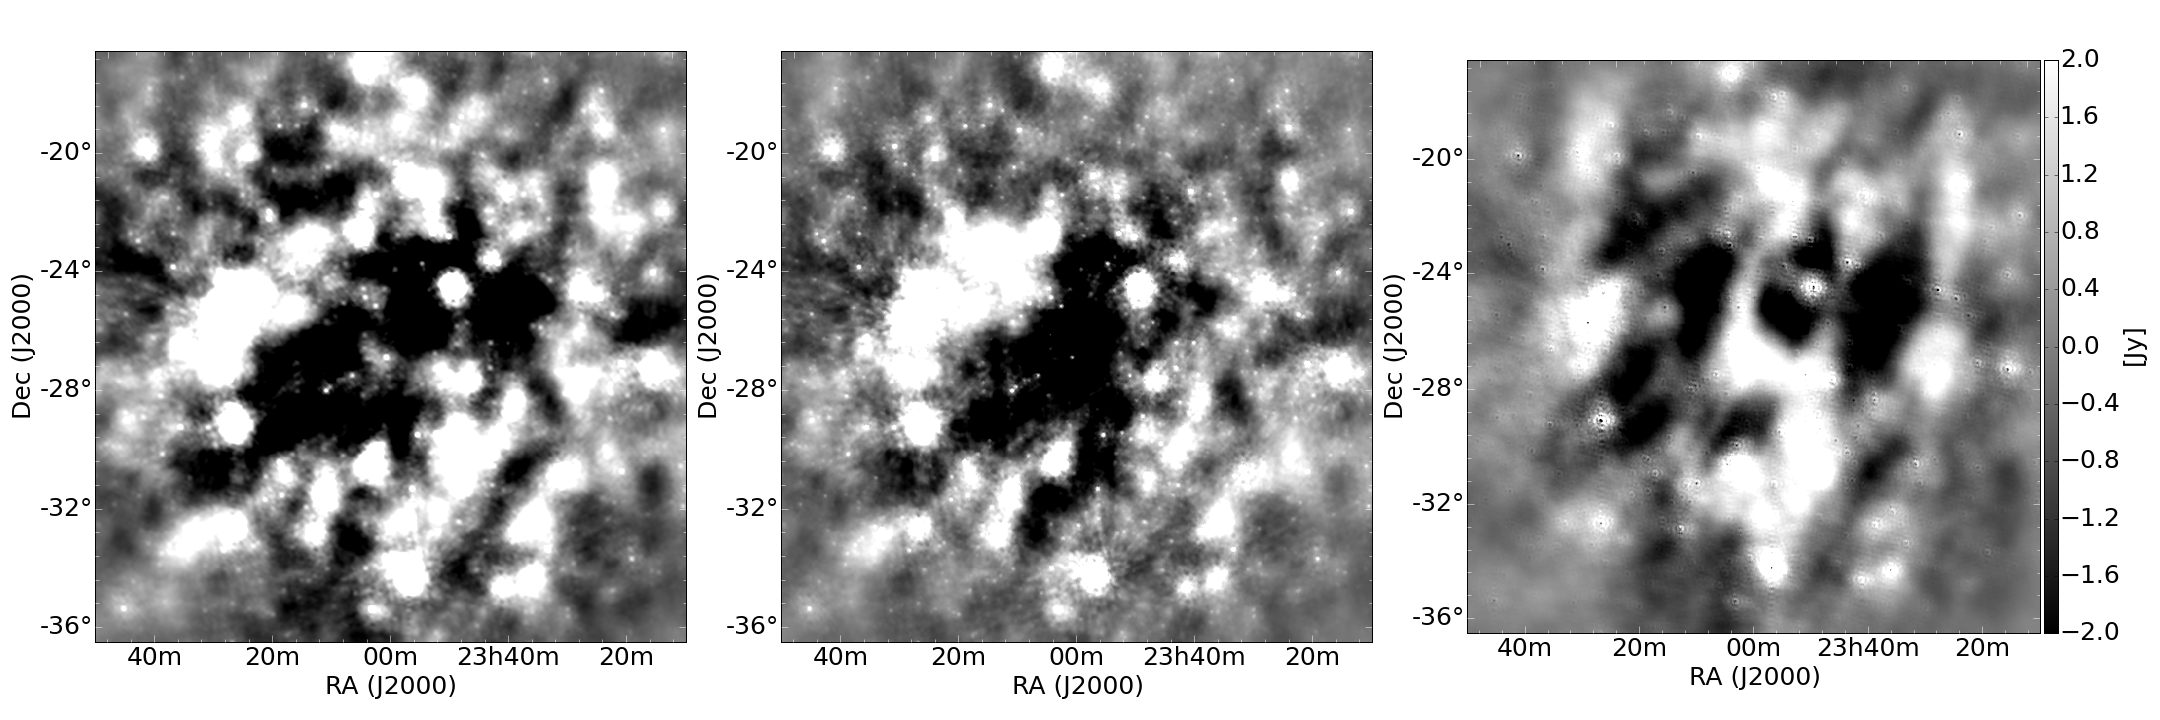
\includegraphics[width=1\textwidth]{figures/FHD_RTS_dirty_compare_31March2015.png}
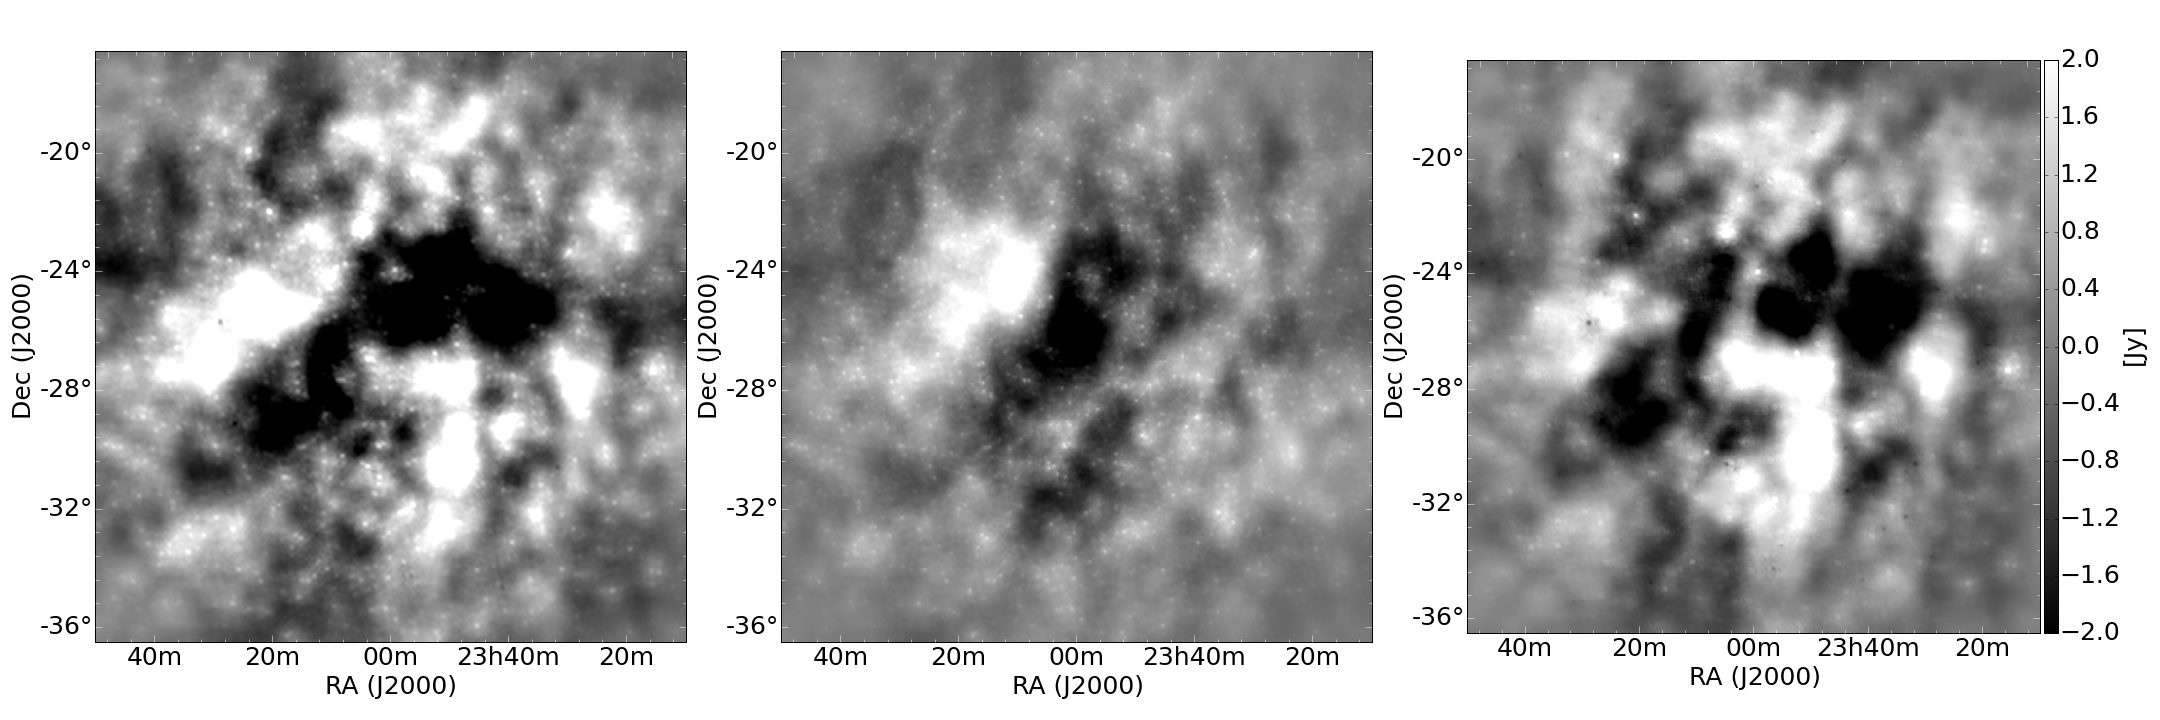
\includegraphics[width=1\textwidth]{figures/FHD_2014c_RTS_March_2015.png}
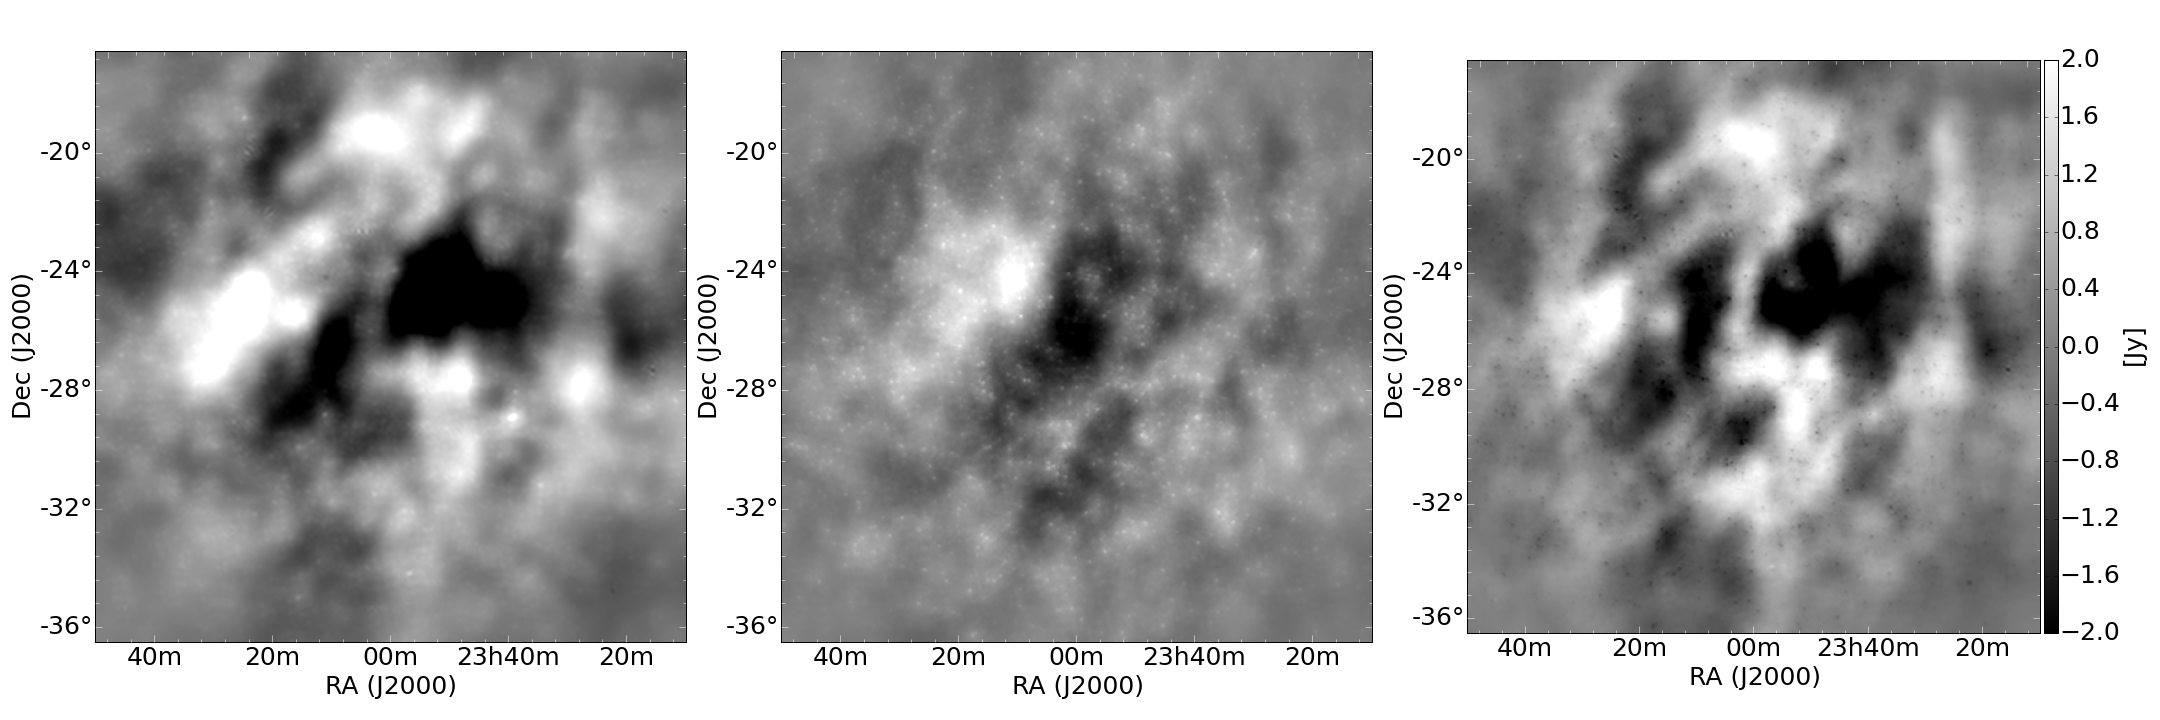
\includegraphics[width=1\textwidth]{figures/FHD_2014c_RTSnominal.png}
\caption{A comparison between the image outputs of the FHD (left), RTS (center) and their difference (right) all averaged in the spectral dimension and projected from native healpix to flat sky.  The images are dirty, in the sense that catalog sources have been subtracted, but no additional deconvolution has been performed.  In the top row, no subtraction has been performed, in the middle row the same catalog of 300 sources have been subtracted, and on the bottom each system is allowed to make its own determination of the appropriate number of sources with FHD increasing the count to \~1000 and RTS staying at 300. Both have been left in the natural weighting used by image-based power spectrum schemes. Most of the $uv$ data points sample scales on the degree or larger scales, thus the greatest differences are apparent at large scales.     \label{fig:image_compare}}
\end{center}
\end{figure*}


\begin{deluxetable}{lccr}
\tablecolumns{4}
\tablewidth{0pt}
\tablecaption{Foreground subtraction image differences }
\tablehead{
\colhead{\parbox{10em}{Number of sources subtracted FHD/RTS}}  & 
\colhead{FHD RMS\tablenotemark{*}} &
\colhead{RTS RMS\tablenotemark{*}}&
\colhead{diff RMS\tablenotemark{*}}
}
\startdata
None/None & 1.97 & 1.49 & 1.08 \tabularnewline
300/300 & 1.19 & 0.59 & 0.991 \tabularnewline
1000/300 & 0.923 &  0.59 & 0.817
%None/None & 1.97 & 1.49 & 1.08 \tabularnewline
%300/300 & 1.19 & 0.66 & 0.991 \tabularnewline
%1000/300 & 0.923 &  0.483 & 0.806
\enddata
\label{tab:image_comparison}
\tablenotetext{*}{The standard deviation of the image in Jy}
\end{deluxetable}

\subsection{Power Spectrum \#1: \eppsilon}
\label{sec:EPPSILON}
\eppsilon calculates a power spectrum estimate from image cubes and directly propagates the error bars through the full analysis and is described more fully in \eppsiloncite. The design criteria for this method is to make a relatively quick and uncomplicated estimate of the power spectrum to provide a quick turnaround diagnostic. The input to \eppsilon is gridded image cubes for  each 112s snapshot, such as are produced by FHD or RTS imaging, in which the data has been split into interleaved time samples (referred to as even and odd cubes) along with matched cubes containing the modeled instrumental weighting and variance. These snapshot healpix cubes are integrated in time keeping pixels with a beam weight of 1\% or more, a cut which effectively limits the field of view to $\sim$20\arcdeg. The accumulated data, weight and variance cubes are Fourier transformed in two dimensions to take them to $uvf$ space where the spatial covariance matrix is assumed to be diagonal. This is a better assumption if the $uv$ pixel size is well matched to the primary beam size so we restrict the spacing of modes in the spatial DFT to be equal to the inverse of the primary beam field of view. The data (variance) cubes are then divided by the weight cubes (weight cubes squared) to arrive at the best estimates of the sky and variances. Next the sum and difference of the even and odd cubes are computed with variances given by adding the reciprocal of the even and odd variances in quadrature. The difference cube then contains only noise (as long as the time interleaving is fine enough) and the sum cube contains both sky signal and noise.

The next step is to Fourier transform in the frequency direction. Here we choose to use the full 30\,MHz spectral window, weighted by a Blackman-Harris window function, which heavily down-weights the outer half of the band to effectively sample 15\,MHz; a cosmological redshift range of 0.86. This weighting scheme minimizes the covariance of bright foreground modes between power spectrum modes as described in \cite{Thyagarajan:2013p10039,Parsons:2012p8896,Vedantham:2012p9026}, among others.  The spectral Fourier transform is dominated by the MWA passband gaps which occur every 1.28\,MHz and imparts a harmonic structure to the $k_\parallel$ dimension.  The Fourier transform of unevenly sampled data is well described by the Lomb \& Scargle method which obtains a periodogram in the trigonometric cross products of ($\sin$,$\cos$), resulting in a two-by-two covariance matrix for each Fourier mode containing the $cos^2$ and $sin^2$ terms on the diagonal and the $cos\times sin$ cross term in the off-diagonal elements. \cite{lomb1976,scargle1982}. Diagonalizing this matrix at each $k_\parallel$ mode finds the best estimate of the power spectrum in the presence of missing data.  The sky signal power is  estimated by the square of the sum cube minus the square of the difference cube, which  is mathematically identical to the even/odd cross power if the even and odd variances are identical, while the square of the difference cube provides a realization of the noise power spectrum. Finally the power cubes are averaged averaged, weighting by variance, in $k_x-k_y$ rings to get to a two dimensional $k_{\|}-k_{\bot}$ space.



% The difference power spectrum provides our noise estimate, which we subtract from the sum power spectrum to estimate an unbiased noise power spectrum.  This is mathematically identical to the cross-power between even and odd if the even/odd variances are identical, which we have verified in this data set.  Finally the 3D power cubes are be averaged (weighted by the variance) in $k_x-k_y$ rings into the  two dimensional $k_{\|}-k_{\bot}$ space shown in the left column of Figure \ref{fig:pspec_compare}.

%The covariance matrix (diagonal in $uvf$); terms given by the sum and difference variances) is propagated through this Fourier transform and covariances between non-identical modes are marginalized over. This results in a two-by-two covariance matrix for each Fourier mode containing the $cos^2$ and $sin^2$ terms on the diagonal and the $cos\times sin$ cross term in the off-diagonal elements. These covariance matrices (and the associated data) are then diagonalized for each Fourier mode (as in \cite{lomb1976} \& \cite{scargle1982}), producing two terms that are squared and combined to get the best power estimates. The sky signal power is best estimated by the square of the sum cube minus the square of the difference cube\footnote{This is mathematically identical to the even/odd cross power if the even and odd variances are identical} while the square of the difference cube provides a realization of the noise in the power spectrum. Finally the power cubes can be averaged (using a variance weighting) in $k_x-k_y$ rings to get to a two dimensional $k_{\|}-k_{\bot}$ space.

\subsection{Power Spectrum \#2: CHIPS}
\label{sec:CHIPS}
The CHIPS power spectrum estimation method computes the maximum likelihood estimate of the 21~cm power spectrum using an optimal estimator formalism and is more completely described in \chipscite.  The design criteria for this method were to fully account for instrumental and foreground induced covariance in the estimation of the power spectrum  The approach is similar to that used by \cite{Liu:2011p8763}, but with the key difference of being performed entirely in $uv$-space, where the data covariance matrix is simpler (block diagonal), and feasible to invert. This approach also allows straightforward estimation of the variances and covariances between sky modes by direct propagation of errors, and requires fewer preparatory analysis steps. CHIPS takes as input calibrated and foreground subtracted time-ordered visibilities. Tapping into the pipeline post-calibration but before imaging CHIPS uses its own internal instrument model to estimate and propagate uncertainty.	

The method involves four major steps: (1) Grid and weight time-ordered visibility channel onto a $uvw$-cube using the primary beam model, (2) compute the least squares spectral (LSS) transform along the frequency dimension to obtain the best estimate of the line-of-sight spatial sky modes (this technique is comparable to that used \eppsilon); (3) compute the maximum-likelihood estimate of the power spectrum, incorporating foregrounds and radiometric noise,  averaging $k_x$ and $k_y$ modes into annular modes on the sky, $k_\bot$; (4) compute the uncertainties and covariances between power estimates. The first step is the most computationally-intensive, requiring processing of all the measured data. The principle departure point for CHIPS from \eppsilon is in the much finer resolution of the $uv$ grid.  Using an instrument model, CHIPS calculates the covariance between $uv$ samples as a function of frequency.  Since the beam and $uv$ sampling function are both highly chromatic, extra precision in this inversion is thought to be highly beneficial. After a line of sight transform similar to that used by \eppsilon, this covariance information is inverted to find the fisher information, the maximum likelihood power spectrum, and covariances between measurements.  The resulting dataset provides an estimate of the power in each $k_\bot,k_\parallel$ mode, shown in the right column of Figure \ref{fig:pspec_compare}. 

%covariance estimates the maximal error bar, Bryna likes marginalization.
% doesn't really do anything to the data. just propagates error bar.  

\subsection{Power Spectrum \#3: Implicit Covariance}
\label{sec:empirical _cov}
%The empirical  covariance method \cite{Liu:2011p8763} postulates the power spectrum residuals are still dominated by non-reionization signals and removes this excess by computing the pixel to pixel $uvf$ covariance (averaged in $uv$ rings, and down-weights by its inverse. The method builds on the optimal estimator framework used in the previous MWA 32T results \cite{Dillon:2014p9788} and in the recent PAPER 64 results \cite{2015arXiv150206016A}.  This final step takes as input FHD calibrated image cubes and a set list refined by jackknifing in \eppsilon, the resulting power spectrum is shown in Figure \ref{fig:1D_pspecs} and is discussed more completely in \dilloncite.  This 1D power spectrum includes the same data shown in Figures \ref{fig:image_compare} and\ref{fig:pspec_compare}. Though well above the predicted signal level the amplitudes 2$\sigma$ error bars are notably consistent with noise.

The quadratic estimator method of \cite{Liu:2011p8763} treats foreground residuals in maps as a form of correlated noise and simultaneously downweights both noisy and foreground-dominated modes, keeping track of the extra variance they introduce into power spectrum estimates. This technique, accelerated by \cite{Dillon:2013p10497}, was used in the previous MWA 32T results \cite{Dillon:2014p9788}.  A very similar technique, working on visibilities rather than maps, was used for the recent PAPER 64 results  \cite{2015arXiv150206016A}.  \dilloncite build on these methods to mitigate errors introduced by imperfect mapmaking and instrument modeling through empirical covariance estimation, assuming all data covariance is sourced by foregrounds after shallow integrations

This final step takes as input FHD calibrated images with foregrounds subtracted as well as possible, split into even and odd time-slices and averaged over many observations using an observation set list curated by examining \eppsilon power spectra. From these cubes, it estimates the frequency-frequency foreground residual covariance in annuli in $uvf$ space, assuming that different uv cells have uncorrelated foreground residuals. This assumption, similar to that made by CHIPS, allows the combined foreground and noise covariance to be inverted directly. The resulting power spectrum, made with the Dillon et al. (2013) fast algorithm and the frequency flagging psuedo-inverse and 2D to 1D binning techniques of Dillon et al. (2014), was used to create the spherically averaged power spectra in Figure 4 which is described in detail in \dilloncite. This 1D power spectrum includes the same data shown in Figures 2 and 3, split into three equal-bandwidth redshift bins. Though well above the predicted cosmological signal level, the measurements are notably consistent with noise across a wide range of $k$. 


\section{Results}
\label{sec:results}
A heuristic comparison of the images and power spectra reveals several consistent features. A comparison of images at several stages of foreground subtraction is presented in Figure \ref{fig:image_compare}. The columns compare between the two pipelines FHD on the left and RTS in the center; the right column shows the difference between the two while the rows are different levels of foreground subtraction. RMS of  each image, a measure of the total power, is given in Table \ref{tab:image_comparison}.  The top row is a comparison before any model subtraction. Presented in the raw weighting, without application of any deconvolution, small differences in weighting schemes are perceptible as slightly different point-spread-functions around isolated sources, and broader response around clusters of sources.  

Foreground subtraction is highly dependent on the choice of sources included in the model: too few sources subtracted leaves an excess of power which must be removed as extra free parameters in the covariance step, too many sources leaves open the possibility of mis-subtraction as the number of sources and amount of sky covered increases. In the middle row we have locked both pipelines to the RTS's smaller but more readily diagnostic catalog of 300 sources.  This subtraction step decreases the image rms by half and results in a somewhat flatter difference image.  In the bottom row we have allowed each system to select from its internal catalog based on nominal operating parameters, for the FHD this means the number of sources increases to 1000 and results in a further decrease in image rms by \~33\% and a smaller 20\% decrease in the {\emph difference} with the RTS image.   This is the residual data set which is passed to the power spectrum estimation portions of the pipelines.

   The primary feature in the two images shown in Figure \ref{fig:image_compare} is that both consistently present a significant amount of large scale power which, while visually similar in some respects, differs at the 50 to 100\% level.  The power is generically described as several large ``islands'' of power (both positive and negative) and which, in the difference image, give the appearance of beginning to dissipate as more sources are subtracted.  


The residual, after subtraction of many hundreds of sources, tells a fairly consistent story of a significant amount of large scale power remaining, though the two imagers disagree somewhat on the exact arrangement.  One possibility follows from a consideration of the physical layout of the MWA and the  approach to calibration used in both imagers.  The MWA configuration is a compact core --with tiles separated by $<5$ wavelengths in some cases-- and a density that falls off radially; a configuration designed to match the expected steep rise of reionization power at large scales. Thus the image weights are highly condensed in the center of the $uv$ plane and make images dominated by large scale structure \cite{Beardsley:2013p9952}; reconstruction of the large scales is crucial to subtracting modeled foregrounds at small $k$, where reionization is brightest.   The primary question is whether any large-scale structure is ``real'', rather than some mis-calibration or other artifact that affects the large number of short baselines.  Calibration errors in a traditional interferometer having uniformly distributed baselines reveal themselves as side lobes around bright point sources; similar errors on the core-heavy MWA reveal themselves as artifactual large-scale power which is more difficult to distinguish from true emission.  In essence, by using only the longer baselines, and a model composed only of point sources, we have performed a calibration on a small amount of data on the periphery of the core and extrapolated the result to the majority of the data at the shortest spacings. It should be no surprise that small differences in calibration and weighting  heavily affect the accuracy of the images.  These differences are also apparent in the power spectrum.
%XXX TODO color scale for the images. How bright is that stuff?









\subsection{Power Spectra}
Application of our two independent power spectrum estimators to our two calibration and foreground subtraction pipes gives us a total of four different power spectra (Figure \ref{fig:pspec_compare}).  Each power spectrum estimator has been developed to target the output from a ``primary'' calibration and foreground subtraction process --the diagonal elements of Figure \ref{fig:pspec_compare}-- and have been highly optimized to that up-stream source of data.  The off-diagonal power spectra were created using auxiliary links which import the data and the metadata produced by the foreground subtraction step.  Since they are less highly optimized, lacking as they do the advantage of a close working relationship, these pathways represent an upper limit on the variance to be expected from small analysis differences and allow us to look for effects common to foreground subtraction.


Properties shared by all are the large amount of power at low $k_{\parallel}$ roughly at an amplitude of $10^15$ mK$^2$/Mpc$^3$ and approximately flat in $k_{\perp}$ and the so-called ``wedge'' shaped linear dependance on baseline length.  The wedge is due to the inherently chromatic nature of a wide field instrument scattering smooth spectrum foregrounds; sources entering far from the phase center appear as pixels at higher $k_\parallel$. The solid and dotted lines in the figure indicate the upper boundaries of power from sources at the horizon and at the beam half power point, respectively.  With the exception of some instrumental features foreground power is well isolated within this expected boundary.

The two main instrumental systematics are horizontal striping due to missing or poorly calibrated data at the edges of regular coarse passbands and vertical striping due to spectral variation in $uvf$ sampling. The former can be minimized by careful calibration of the passband, the latter by $uv$ rotation synthesis and by accounting for covariance between $uvf$ samples. 

The most noticeable difference between foreground removal methods is in the shape of the power spectrum at $k_\parallel=0$.  Where power spectra using data from FHD have a fairly uniform increase in power with decreasing $k_\perp$ those using RTS data have a roughly flat spectrum which increases dramatically in the few bins below $k_\perp<.002$ or below 20 wavelengths.  This corresponds to power on scales of 2.86 \arcdeg. The number of baselines drops precipitously below 20 wavelengths.XXX 

The major difference between the power spectrum methods is in the calculation and minimization of $uvf$ covariance.   CHIPS aims to make a more accurate mathematical treatment of the covariance but to do so it must take on more of the instrument modeling. Meanwhile, \eppsilon leaves the modeling to the foreground subtraction step and assumes that, to first order, covariance has been minimized by an  additional down-weighting by the primary beam of the instrument;  i.e. $uv$ cells are chosen to be sized by the inverse of the primary beam width.  Thus one of the largest differences is in the amount of correlation along the vertical, or line-of-sight, direction.  Both CHIPs and \eppsilon, when applied to their  primary foreground subtraction strategy (FHD for \eppsilon and RTS for CHIPS), have minimal line-of-sight covariance at low $k_\perp$ where frequency to frequency variation in $uv$ sampling is small. At high $k_\perp$ \eppsilon's simplistic Fourier Transform reveals the large residual correlation between different $uv\eta$ cells caused by the fact that baseline length changes quickly with frequency.  \eppsilon has so far avoided directly accounting for covariance choosing speed over accuracy on long baselines.

{\bf XXX TBD add a little discussion of the differences between power spectra when things are getting closer to finalize: focus on 1) things depending on calibration/foreground subtraction, 2) things depending on power spectrum calc.  3) things arising from correlation between fg and ps (probably due to interface stuff like weights or whatever)}


Using the speedup provided by \eppsilon, many iterations of ``preview'' power spectra were used to view the effect of calibration and flagging choices on the power spectrum. For example the wide-field effects, described in detail by \cite{2015arXiv150207596T}, are clearly visible in power spectra computed by \eppsilon and are seen to be stronger for certain configurations of pointing and sky. Removing these portions of the data eliminated a substantial amount of bleed from the wedge into the window.  Using this and other jackknife selections we arrived at a refined data FHD image cube which was then carried into the \empirical cov analysis resulting in the power spectra shown in Figure \ref{fig:1D_pspecs}.   Though well above the predicted signal level the 2$\sigma$ error bars are mostly consistent with noise.   Residual excesses --particularly near low $k$s--  are consistent with a fairly aggressive inclusion of points near to the wedge, in this case points up to 0.02$Mpc^{-1}$ away from the horizon (the solid black line in Figure \ref{fig:pspec_compare})were included.

\begin{figure*}[h!]
\begin{center}
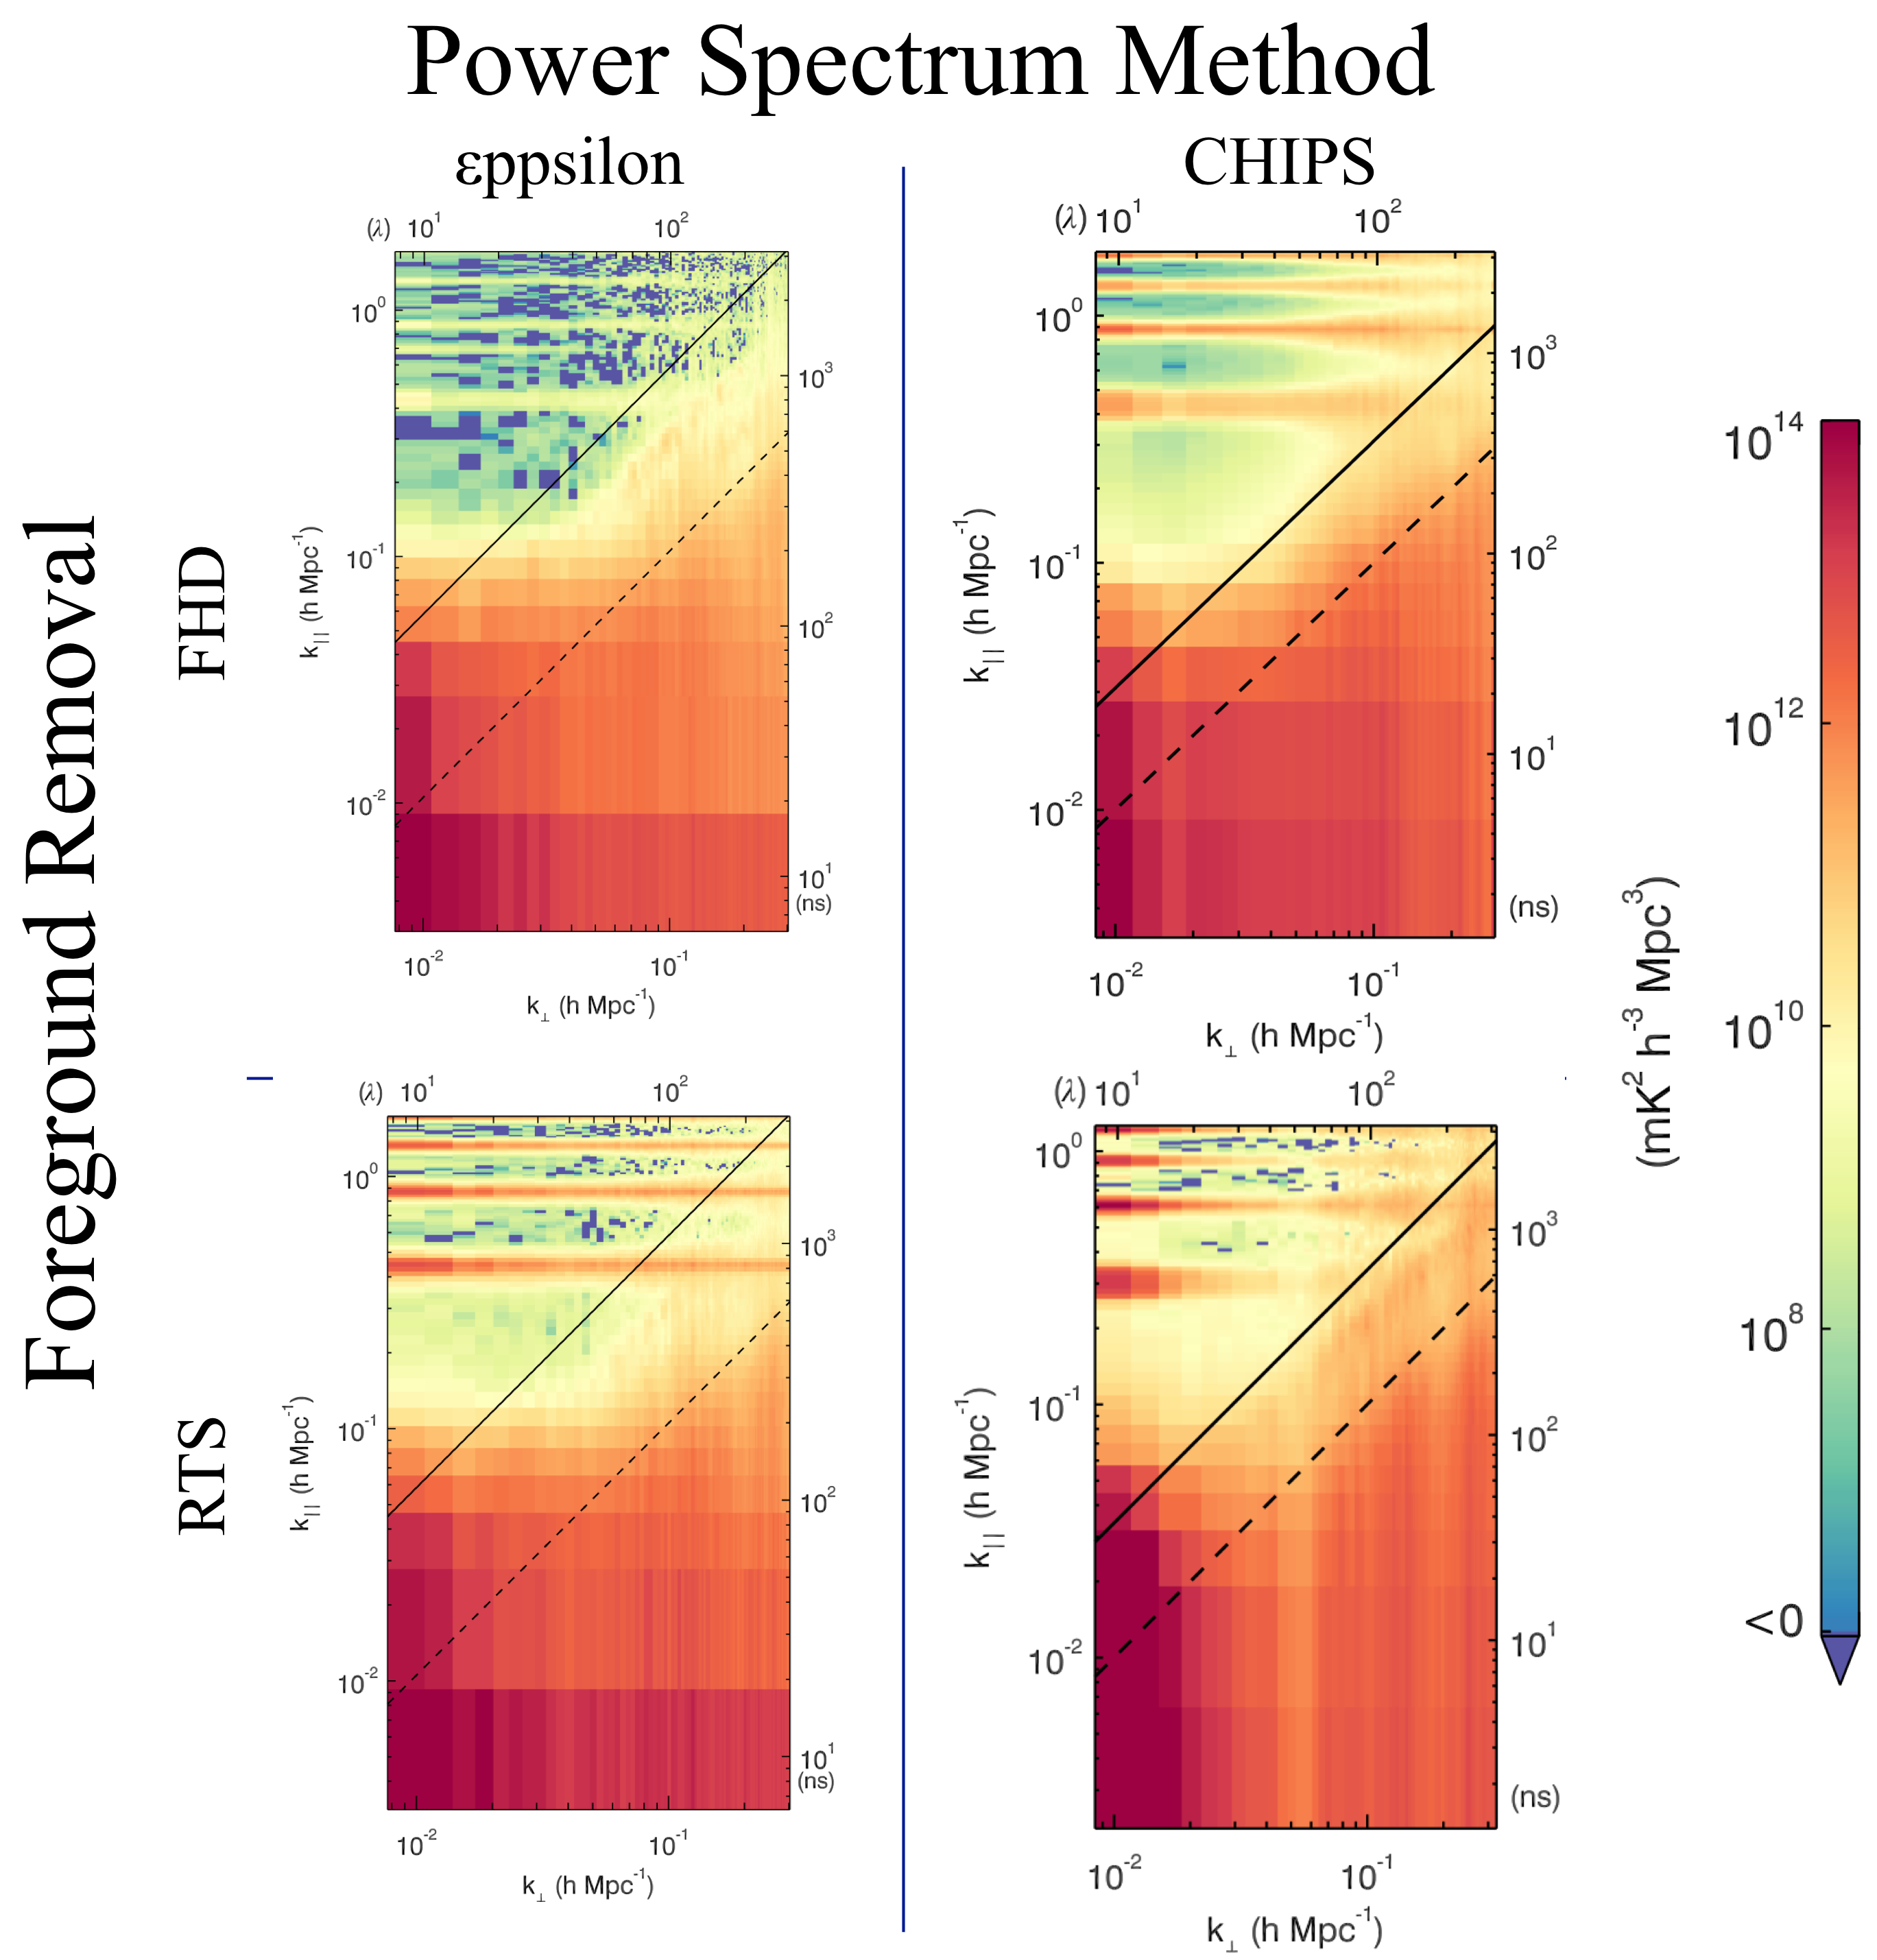
\includegraphics[width=0.8\textwidth]{figures/MWA_PS_compare/MWA_PS_compare.png}
\caption{MWA power spectra computed using two foreground subtraction methods and two power spectrum estimation methods.  In the top row data have been calibrated to a catalog followed by subtraction of a deeper catalog modeled into instrumental space using the Fast Holographic Deconvolution method, in the bottom row calibration and foreground subtraction have been performed with the MWA Real Time System.  In the left column, power spectra have been estimated with \eppsilon, which emphasizes speed and full error propagation, in the right column, CHIPS tries to minimize correlation between $k$ modes.\label{fig:pspec_compare}}
\end{center}
\end{figure*}


\begin{figure*}[h!]
\begin{center}
\includegraphics[width=\textwidth]{figures/1dDeltaSqComparisonFHD.pdf}
\caption{Here we have power spectra averaged along shells of constant $|k|$ where foregrounds have been further down-weighted by inverse covariance after calibration and foreground subtraction by FHD. In three hours of data, two independent methods demonstrate similar, largely noise limited, measurements of the power spectrum.  A theoretical model (blue) sets the scale.  The red points are weighted by an empirical estimate of foreground-like covariance and are further described in \dilloncite.  The black points are computed using the CHIPS estimator and then further weighted by a model of the confused foregrounds and are further described in \chipscite. The action of both foreground down-weighting schemes is to decrease the amount of power leaking from the very lowest $k$ modes; at low $k$ CHIPS finds somewhat higher power than the Dillon scheme.  The very high CHIPS point  is dominated by a very small amount of data, but is included for completeness.  At high $k$ values both methods are in good agreement with each other and with theoretical noise level (omitted for clarity); given the data included we expect a $\sqrt{2}$ difference in the noise level.  Any remaining excesses in this plot are thought to be consistent with a fairly aggressive inclusion of points near to the wedge --in this case points up to 0.02Mpc$^{-1}$ away from the horizon (the solid black line in Figure \ref{fig:pspec_compare}) were included-- and known systematics like cable reflections.\label{fig:1D_pspecs}}
\end{center}
\end{figure*}


\section{Conclusions}
\label{sec:conclusion}
      Each pipeline is necessarily built on a complex software framework which is only imperfectly described in prose and is susceptible to human error.  Comparison of both 2D images and 3D power spectra have allowed us to build confidence in our estimate of the power spectrum and have revealed a number of issues both systematic (related to our understanding of the instrument or foregrounds) and algorithmic (optimizing our use of this knowledge). Lessons learned include:
\begin{itemize}
\item in-field calibration vs calibration transfer
Comparison of RTS and FHD images continues to reveal the significance of calibration algorithm as well as weighting schemes on the effectiveness of imaging and model subtraction.  Differences remaining in the images presented here are likely due to small divergences in calibration method. Current work focuses on finding a robust calibration model upon which the two systems agree and results in better subtraction of the sky model.

\item cable reflections
One debatable aspect of calibration is the number of free parameters allowed into the spectral dimension. Individual calibration of each channel independently allows the greatest flexibility but has the consequence of possibly adding or subtracting to the spectral line reionization signal.  Both calibration pipelines begin by calibrating each channel and then fitting a spectral average.  The RTS fits a low order polynomial, piecewise, to each of the 24 1.28MHz sub-band solutions, while FHD fits a similar order polynomial to the entire  band's calibration solution.  Inspection of power spectra calibrated using the FHD scheme revealed  previously unknown spectral features corresponding to reflections on the analog cables at the -20dB level (~1.5\%). FHD calibration now includes a fit for these reflections and the feature is no longer visible. These features are fully covered by the RTS fit (which uses of order 10 times as many free parameters as FHD).

\item full forward modeling for absolute calibration, signal loss
One way in which all pipeline results differed from each other is in the overall amplitude of the power spectrum scale. Agreement only occurs when flux scale, weightings, and fourier conventions are all in alignment.  Perhaps the most important factor is assessment of signal loss.  Unintential or unavoidable down-weighting or subtraction of reionization signal could occur at multiple stages such as bandpass calibration, $uvf$ gridding, or inverse covariance weighting. This loss is best calibrated via forward modeling of a simulated reionization signal and in the process provides verification of the overall power spectrum scale.  Such simulations have been used to verify the various steps in the FHD-\eppsilon pipeline and by stepping through the pipeline at each major operation have been shown to be self-consistent (see \eppsiloncite) and suitable for calibration of the other pipelines.
\end{itemize}

Through the comparison process we have seen the many ways a single analysis pipeline can error.  Only by comparing multiple redundant pipelines has it been possible to have confidence in the results of any one pipe.


In this overview paper we have provided a top level view of foreground subtraction and power spectrum estimations methods described more completely in companion papers \eppsiloncite, \chipscite, and \dilloncite and provided a basis for an apples-to-apples comparison.  In this comparison we see that both foreground subtraction methods are able to reliably remove about 50\% of the power with a fairly simplistic model but that the reconstruction of the residual large scale power depends heavily on small differences in calibration and imaging algorithm which ultimately limits the accuracy of the reconstruction.  In a similar way we use the difference between two independently developed power spectrum pipelines to reveal effects in the power spectrum which seem to be unique to the power spectrum estimation, those common to the calibration and foreground subtraction step, and those which appear to be common to the sky itself and on a believably consistent scale.  Though none of the power spectra are identical, the degree of agreement and the success at making nearly noise limited measurements allows us to draw conclusions about the relative quality of different selections of data.  Bad data is truly bad and not evidence of an underlying software or algorithmic problem.  Using our validated pipeline to make quick estimates of the power spectrum in different selections of data we were able to select a high quality set, with a well understood calibration, for application of the empirical  covariance technique and generate a noise limited measurement. 

The 1D power spectrum presented here and in \dilloncite is roughly a 500 times deeper then the previous MWA power spectrum \cite{Dillon:2014p9788} which was done using roughly the same amount of integration time but only 32 of the present 128 tiles.  Future work will focus on refining calibration and weighting schemes to more accurately reconstruct large scale power and building on deeper integrations using data collected in recent observing campaigns.




\acknowledgments

This work was supported	 by the U. S. National Science Foundation (NSF) through award AST--1109257. DCJ is supported by an NSF Astronomy and Astrophysics Postdoctoral Fellowship under award AST--1401708. JCP is supported by an NSF Astronomy and Astrophysics Fellowship under award AST-1302774. This work makes use of the Murchison Radio-astronomy Observatory, operated by CSIRO. We acknowledge the Wajarri Yamatji people as the traditional owners of the Observatory site. Support for the MWA comes from the NSF (awards: AST-0457585, PHY-0835713, CAREER-0847753, and AST-0908884), the Australian Research Council (LIEF grants LE0775621 and LE0882938), the U.S. Air Force Office of Scientific Research (grant FA9550-0510247), and the Centre for All-sky Astrophysics (an Australian Research Council Centre of Excellence funded by grant CE110001020). Support is also provided by the Smithsonian Astrophysical Observatory, the MIT School of Science, the Raman Research Institute, the Australian National University, and the Victoria University of Wellington (via grant MED-E1799 from the New Zealand Ministry of Economic Development and an IBM Shared University Research Grant). The Australian Federal government provides additional support via the Commonwealth Scientific and Industrial Research Organisation (CSIRO), National Collaborative Research Infrastructure Strategy, Education Investment Fund, and the Australia India Strategic Research Fund, and Astronomy Australia Limited, under contract to Curtin University. We acknowledge the iVEC Petabyte Data Store, the Initiative in Innovative Computing and the CUDA Center for Excellence sponsored by NVIDIA at Harvard University, and the International Centre for Radio Astronomy Research (ICRAR), a Joint Venture of Curtin U
\bibliography{bibliography/library}

\end{document}

